\chapter{\uppercase{Generador fotovoltaic i inversor}}
Un generador és una màquina, aparell o dispositiu que produeix energia elèctrica amb una tensió i un corrent d'unes característiques determinades. L'adjectiu fotovoltaic s'usa per designar aquells sistemes en què es produeix una força electromotriu entre dos metalls que estan en contacte i exposats a una radiació electromagnètica.\\
\newline Un conjunt de panells solars connectats entre sí ja sigui en sèrie, en paral·lel o amb associació sèrie-paral·lel es pot considerar un sol generador fotovoltaic.\\
\newline Un panell solar ve definit per diferents paràmetres que s'han de tenir en compte a l'hora de dissenyar una instal·lació. Prèviament cal determinar la quantitat de panells de la instal·lació en funció de l'energia que es vol produir.

\section{Potència de la instal·lació fotovoltaica}
S'ha calculat al capítol anterior que el consum total de l'habitatge al cap de l'any és de 5.504 KWh.\\
\newline Es proposa instal·lar les plaques necessàries per generar al cap d'un any un  valor d'energia inferior però proper a l'energia consumida aquell any a l'habitatge. D'aquesta manera hi haurà moments en què tota l'energia elèctrica generada serà igual a la consumida a l'habitatge, altres en què els excedents es lliurin a la xarxa i altres en què les plaques no generin i s'hagi de consumir únicament energia de la xarxa.\\
\newline Es proposa utilitzar un panell amb un eficiència del 17\% i una superfície de 1,94 $m^2$. Amb aquestes dades i coneixent el valor de la irradiació global es determina que un sol panell donarà 517,73 kWh al cap de l'any. 10 panells d'aquest model donaran 5.177 kWh anuals, valor molt proper al d'energia consumida anual a l'habitatge.\\
\newline Cal tenir en compte les ombres generades per l'edifici del costat sud i els arbres d'aquest mateix costat, que tenen una altura superior a la de la casa del projecte. La imatge de la Figura \ref{fig: ombres} s'ha construït a partir de dades reals i a partir de l'IDAE.
\begin{figure}[H]
\begin{center}
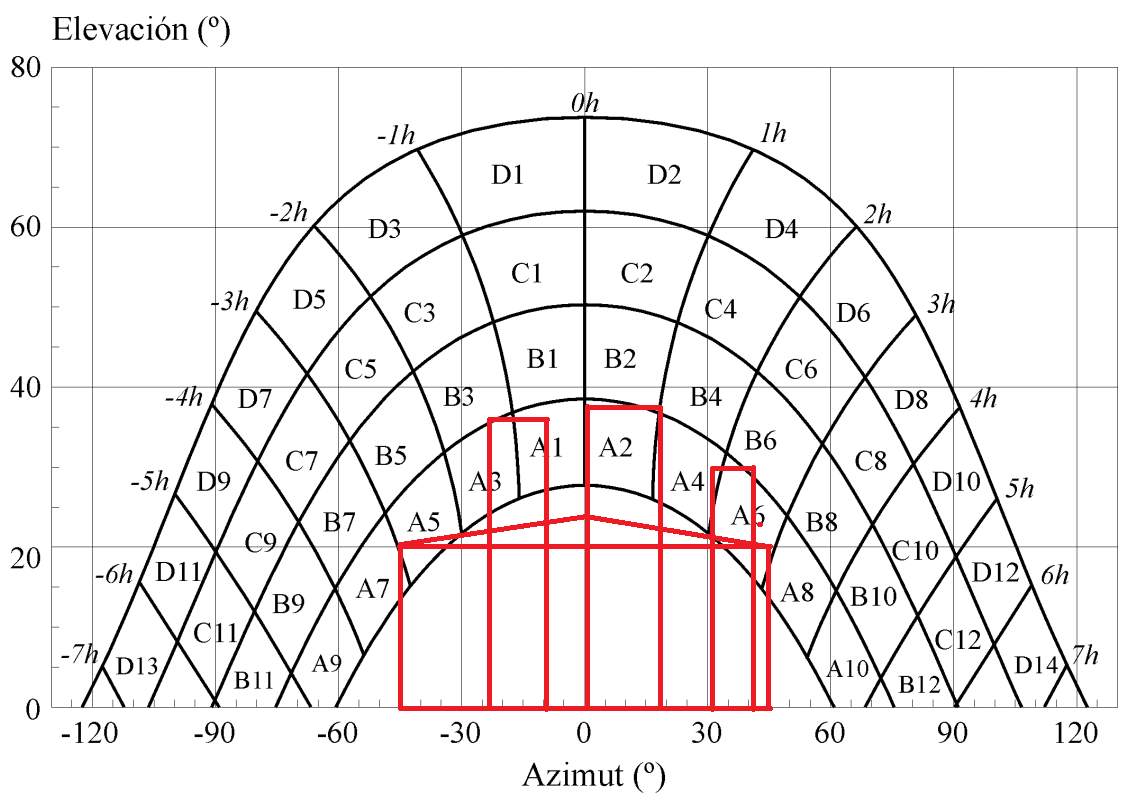
\includegraphics[scale=0.45]{images/o2.png}
\end{center}
\caption{Mapa d'ombres}
\label{fig: ombres}
\end{figure}

\noindent Degut a la inclinació i orientació de les plaques es fa servir la taula 5-A de l'IDAE, per tal de determinar el factor d'ombrejat (FS). Segons l'IDAE cal identificar si cada casella té un 0\%, un 25\%, un 50\%, un 75\% o un 100\% de la seva superfície coberta.\\
\newline La Taula \ref{tab:ombres} mostra el percentatge de superfície de cada casella, el valor de pèrdua tabulat de l'IDAE i la pèrdua que ocasiona cada casella. Així, es dona un total, el factor d'ombrejat (FS).
\begin{table}[H]
\small
  \centering
    \begin{tabular} {|l|r|r|r|}
 \hline  
 \multicolumn{1}{|l|}{Casella} &  \multicolumn{1}{r|}{Factor de superfície} &  \multicolumn{1}{r|}{Sombrejat casella al 100\%} &  \multicolumn{1}{r|}{Sombrejat casella} \\ \hline \hline
A5 & 0,25 & 1,84 & 0,46 \\ \hline
A3 & 0,5 & 2,70 & 1,35 \\ \hline
A1 & 0,5 & 3,15 & 1,58 \\ \hline
A2 & 1,0 & 3,17 & 3,17 \\ \hline
A6 & 0,75 & 1,79 & 1,34 \\ \hline \hline
Total & \multicolumn{3}{r|}{7,90} \\ \hline

    \end{tabular}%
    \caption{Sombrejats}
    \label{tab:ombres}
%\caption{Estances de l'habitatge unifamiliar}
\end{table}%

\noindent El total de 7,9\% entra dins els marges que marca l'IDAE, el qual indica que per instal·lacions de propòsit general el màxim per ombres és del 10\%.\\
\newline El factor d'ombrejat (FS) ve donat per l'Equació \ref{fs}.
\begin{equation} \label{fs}
FS = 1-Perdues \ per \ ombrejat
\end{equation}

\noindent El factor d'ombrejat val 0,921. Per tant, el total d'energia generada al cap de l'any baixa a 4.768 kWh.\\
\newline El factor d'irradiació és 1 perquè es pren l'angle òptim d'inclinació i l'angle d'orientació coincideix amb el sud.

% Per tal de determinar els panells solars escollits, abans necessitem conèixer la radiació que incideix sobre la teulada al llarg de l'any. Per fer-ho es consulta un servei web anomenat Photovoltaic Geographical Information System, de la Comissió Europea. El servei determina que, donades les coordenades de l'habitatge, el més òptim és inclinar les plaques amb un angle de 38$^\circ$ respecte la horitzontal i un angle de -3$^\circ$ respecte l'Azimut.

\section{Panell solar escollit}
El panell solar proposat s'anomena GCL-P6/72. Segons el fabricant és d'alta eficiència ja que pot arribar a tenir un 17\% de rendiment. La seva potència màxima, o potència de pic, és de 330 W. El fabricant indica que el rendiment dels panells disminueix de forma lineal al llarg del temps; al cap de 25 anys s'espera un rendiment d'un 80,7\%.\\
\newline Cal dir que aquests 330 W es poden haver aconseguit en condicions idònies que només es donen al laboratori. El mateix fabricant ens indica que per una irradiació de 800 W/$m^2$ la potència màxima és de 237,71 W.\\
\newline A continuació, a la Taula \ref{tab:panell_ideal}, s'indiquen les característiques elèctriques del panell en condicions idònies, per les quals es dona la potència de 330 W.

\begin{table}[H]
\small
  \centering
    \begin{tabular} {|l|r|}
 \hline  
 \multicolumn{1}{|l|}{Característica del panell GLC-P6/72 330 W, condicions ideals} &  \multicolumn{1}{r|}{Valor} \\ \hline \hline
	Potència màxima ($P_{max}$) & 330,00 W \\ \hline
	Tensió a la potència màxima ($V_m$) & 37,80 V \\ \hline
	Intensitat a la potència màxima ($I_m$) & 8,73 A \\ \hline
	Tensió de circuit obert ($V_{oc}$) & 46,20 V \\ \hline
	Corrent de curtcircuit ($I_{sc}$) & 9,33 A \\ \hline
	Eficiència & 17,00 \% \\ \hline
    \end{tabular}%
    \caption{Dades del panell amb irradiació de 1.000 W/$m^2$ i 25 C$^\circ$ de tempratura ambient}
    \label{tab:panell_ideal}
%\caption{Estances de l'habitatge unifamiliar}
\end{table}%

\noindent En condicions més comunes i no tan ideals la potència disminueix considerablement, com s'indica a la Taula \ref{tab:panell_habitual}.\\
\newline Després de consultar a Internet s'observa que a la zona geogràfica en què es pretén instal·lar les plaques la irradiació pot prendre valors de l'ordre de 800 W/$m^2$ com a màxim. Rebre 1.000 W/$m^2$ no seria gens comú.\\
\newline El mes de novembre, per exemple els pics d'irradiació que es reben són d'uns 600 W/$m^2$.

\begin{table}[H]
\small
  \centering
    \begin{tabular} {|l|r|}
 \hline  
 \multicolumn{1}{|l|}{Característica del panell GLC-P6/72 330 W, condicions no ideals} &  \multicolumn{1}{r|}{Valor} \\ \hline \hline
	Potència màxima ($P_{max}$) & 237,71 W \\ \hline
	Tensió a la potència màxima ($V_m$) & 34,50 V \\ \hline
	Intensitat a la potència màxima ($I_m$) & 6,89 A \\ \hline
	Tensió de circuit obert ($V_{oc}$) & 42,90 V \\ \hline
	Corrent de curtcircuit ($I_{sc}$)& 7,58 A \\ \hline

    \end{tabular}%
    \caption{Dades del panell amb irradiació de 800 W/$m^2$ i 20 C$^\circ$ de tempratura ambient}
    \label{tab:panell_habitual}
%\caption{Estances de l'habitatge unifamiliar}
\end{table}%

\noindent Un altre punt a destacar de la irradiació és que aquesta se sol donar en termes d'energia al cap del dia i no pas de potències. De totes maneres, se seguirà parlant de potències ja que és més pràctic. No s'ha d'oblidar, però, que aquesta potència de 800 W/$m^2$ només es pot donar a l'estiu i en moments de molta irradiació. En les demés hores aquesta potència serà molt menor.

%comentar com es decideix la potència que fa falta
%https://assets.leroymerlin.es/is/content/lmes/82165089-0170q-es/mod-fotovoltaico-gcl-330w.pdf


\section{Associació de plaques} %passar model i tal a annex?
Es decideix associar les plaques amb dues branques de 5 plaques per branca, de manera que es combina l'associació sèrie i paral·lel a la vegada. Per entendre millor aquest apartat es considera important conèixer el model dels panells solars, indicat a la Figura \ref{fig:model}.
\begin{figure}[H]
\begin{center}
\begin{tikzpicture} %http://www.texample.net/media/tikz/examples/TEX/power-electronics-rectifier.tex
    \draw
	(0,0)
	to [I=, l=$I_{PV}$] ++ (0,4)
	(2,4)
	to [D] ++(0,-4)
	(4,0)
	to[R=$R_{sh}$] ++(0,4)

    (0,0) to[short, -o] (7,0)
    (0,4) to[short, current/distance=0.5] (4.5,4)
    to[R=$R_{s}$] (5.5,4)
    to[short, i=$I_{out}$, -o] (7,4)
    
        (8,4)
        to[open, v^=$V_{out}$] ++(0,-4)
;
\end{tikzpicture}
\end{center}
\caption{Model d'un panell solar fotovoltaic}
\label{fig:model}
\end{figure}

\noindent $I_{PV}$: corrent que lliura el mòdul.\\
$R_{sh}$: resistència en paral·lel del panell.\\
$R_{s}$: resistència de contacte del connexionat del panell.\\
$I_{out}$: corrent de sortida.\\
$V_{out}$: tensió de sortida.\\
% 
\newline La corba característica $V_{out}$-$I_{out}$ dels panells solars s'obté d'aquest model i dona una intensitat lineal per un gran rang de tensions de sortida. Per altes tensions de sortida la intensitat de sortida és bastant petita. L'inversor intenta treballar en el punt de màxima potència, anomenat MPPT.\\
\newline Les corbes del panell segons el fabricant són les indicades a la Figura \ref{fig:vi}.
\begin{figure}[H]
\begin{center}
\includegraphics[scale=0.3]{images/corba.png}
\end{center}
\caption{Corbes V-I GLC-P6/72 330 W}
\label{fig:vi}
\end{figure}


\noindent Al connectar diversos panells en sèrie pot passar que algun panell consumeixi energia. Això és molt notori quan hi ha ombres, ja que a algunes plaques els incideix el Sol i lliuren una quantitat considerable d'intensitat mentre que les que estan a l'ombra donen molta menys intensitat. Com que estan connectades en sèrie, la intensitat ha de ser la mateixa. A la placa ombrejada, per tant, li passarà molta intensitat a través de $R_{sh}$. Aquesta resistència té un valor considerable. L'hi poden passar uns quants amperes i pot dissipar potències elevades.\\
\newline En cap cas interessa que un panell consumeixi energia enlloc de generar-ne. Com ja s'ha comentat, a la casa objecte d'aquest projecte s'ha observat que és habitual que es projectin ombres a la teulada, ja sigui pels alts arbres que hi ha properament o per les cases de més alçada que la del projecte.\\
\newline Per solucionar el problema una solució tradicional ha estat connectar díodes en paral·lel als terminals de les plaques. L'inconvenient és que aquests díodes tenen una caiguda de tensió de 0,7 V o 0,4 V si són díodes Schottky. Per una intensitat de branca de 7 A, que es podria donar per les plaques escollides, i considerant que múltiples plaques podrien estar ombrejades, es dissiparia una potència petita però considerable. A més, s'escalfarien els díodes. Aquests díodes es troben dins una petita caixa; l'escalfament els pot arribar a deteriorar i disminuir la robustesa de la instal·lació.\\
\newline Es decideix escollir un díode SM74611, o com diu el fabricant, un díode de derivació intel·ligent. De fet, se'n connectaran sis a cada placa.\\
\newline El panell GLC-P6/72 330 W té 6 files de 12 cel·les cadascuna. S'opta per col·locar un díode en paral·lel amb cada fila. Així, pot haver-hi alguna cel·la ombrejada però la resta del panell pot seguir generant energia.\\
\newline Els díodes SM74611 tenen una caiguda de tensió de 26 mV o menys a 7 A. Es pot afirmar que d'aquesta manera la pèrdua d'energia és mínima. \\
\newline El cost d'un díode és del 2\% aproximadament respecte el del panell.\\
%
%
\newline Un cops justificats els díodes, es poden fer els càlculs per conèixer la tensió i la intensitat màximes de sortides de la instal·lació fotovoltaica a partir de la tensió de circuit obert i a partir de la intensitat de curtcircuit. Aquestes dades es mostren a la Taula \ref{tab:maxs}.

\begin{table}[H]
\small
  \centering
    \begin{tabular} {|l|r|}
 \hline  
 \multicolumn{1}{|c|}{Característica} &  \multicolumn{1}{c|}{Valor} \\ \hline \hline
	Tensió màxima ($V_{max}$) & 256,87 V \\ \hline
	Intensitat màxima per branca & 9,56 A \\ \hline
    \end{tabular}%
%    \caption{Màxims de l'associació sèrie dels panells}
%\caption{Estances de l'habitatge unifamiliar}
\caption{Paràmetres màxims resultants de l'associació de plaques}
\label{tab:maxs}
\end{table}%

\noindent S'ha tingut en compte l'efecte de la temperatura. El fabricant dona uns factors per calcular els pitjors casos. A l'annex de càlculs es detallen.
%Díode SM74611
%http://www.ti.com/lit/ds/symlink/sm74611.pdf

\section{Inversor}

L'inversor escollit és un FRONIUS Primo 3.0-1. És costós en comparació a altres equips amb la mateixa funcionalitat però alhora molt fiable.\\
\newline Seguidament s'adjunta la Taula \ref{tab:inversor} amb algunes de les característiques més rellevants de l'inversor. L'equip és adient per la instal·lació de plaques i l'associació d'aquestes que es proposa. En cap cas se superen els màxims que fixa el fabricant de l'inversor. La potència del Fronius Primo 3.0-1 és correcta per la potència màxima que ens poden donar els panells fotovoltaics.
\begin{table}[H]
\small
  \centering
    \begin{tabular} {|l|r|} \hline
  \multicolumn{1}{|c|}{Característica} &  \multicolumn{1}{c|}{Valor}\\ \hline \hline
	Màxima corrent d'entrada ($I_{dc \ max}$) & 12 / 12 A \\ \hline
	Màxima corrent de curtcircuit & 18 / 18 A \\ \hline
	Rang màxim de tensió d'entrada CC ($U_{cc \ min}$ - $U_{cc \ max}$) & 80 - 1.000 V \\ \hline
	Tensió mínima de posada en marxa ($U_{dc \ arranc}$) & 80 V \\ \hline
	Nombre d'entrades CC & 2 + 2 \\ \hline
	Potència nominal AC ($P_{ac,r}$) & 3.000 W \\ \hline
	Acoblament a la xarxa ($U_{ac,r}$) & 1 NPE 230 V \\ \hline
	
    \end{tabular}%
  \label{tab:addlabel}%
  \caption{Característiques de l'inversor FRONIUS Primo 3.0-1}
  \label{tab:inversor}
 \end{table}%

\noindent Per començar a funcionar l'inversor necessita un mínim de 80 V. Si de dia un o dos panells estan ombrejats i la resta no, l'inversor pot seguir funcionant i lliurant energia.\\
\newline Els rendiments de l'inversor són molt elevats, per un gran rang de treball el rendiment és del 95\% o més. En cap cas el rendiment baixa del 80\%.\\
\newline El fabricant indica que l'inversor intenta donar sempre la màxima potència mitjançant el seu sistema de Dynamic Peak Manager, això vol dir que adapta la seva impedància per fer que el producte de tensió i intensitat sigui màxim.\\
\newline Aquest inversor és fàcil de muntar gràcies a què es pot desmuntar en dues parts: la fixa que va a la paret i és on es realitzen les connexions i la de potència, que pesa 21,5 kg. Primer es munta la part fixa, es realitzen les connexions, i després s'acobla la part de potència.\\
\newline Fronius indica que el Primo 3.0-1 és un equip pensat pel futur, per xarxes elèctriques intel·ligents. Hi ha la possibilitat de comunicar l'inversor per interfícies molt diverses com Modbus RTU, Fronius Solar API, Ethernet...\\
\newline S'opta per connectar l'inversor a Internet mitjançant un cable Ethernet. D'aquesta manera el client podrà visualitzar la generació d'energia elèctrica dels seus panells. La web que ofereix Fronius és entenedora i fàcil d'utilitzar.\\
\newline Gràcies a la web de Fronius i a la web que s'explica al següents capítols el client podrà visualitzar dades dels panells i tenir una molt bona idea de com estan funcionant.\\
\newline L'inversor donarà les dades de tensió, intensitat i potència generada, però no pot saber com està treballant cada panell. Per això hi ha la placa electrònica, la qual llegirà les tensions de cada panell, amb les quals l'usuari podrà determinar si els panells estan ombrejats, curtcircuitats o en funcionament normal.




\clearpage


% Table generated by Excel2LaTeX from sheet 'Hoja1'
%\begin{table}[H]
%  \centering
%    \begin{tabularx} {\textwidth} {|X|r|} \hline
%  \multicolumn{1}{|c|}{Descripció} &  \multicolumn{1}{c|}{Quantitat}\\ \hline \hline
%
 %   Placa GLC 330 W & 10 \\ \hline
%    Inversor FRONIUS Primo 3.0-1 Light 3kW & 1 \\ \hline
%    Metres cable Ethernet RJ-45 CAT 8 & 10 \\ \hline
%    Metres cable 4 m$m^2$ PVC & 45 \\ \hline
 %   Metres cable 1,5 m$m^2$ PVC & 100 \\ \hline
 %   Punteres Enghofer E 4-10, 4 m$m^2$, 10 mm & 20 \\ \hline
 %   Punteres Enghofer E 1.5-10 1,5 m$m^2$ 10 mm & 12 \\ \hline
 %   Cinta aïllant 10 m 1,6 cm & 3 \\ \hline
 %   Caixa estanca Solera CONS 100x100x55 mm & 2 \\ \hline
  %  Canal Euroquint 25,16 mm 1,5 metres & 20 \\ \hline
%    Curva canal VECAMCO & 10 \\ \hline
%    Paquet de 50 brides 200x2,6  mm & 2 \\ \hline
%    Regleta nylon 12 pols 16 mm & 4 \\ \hline
%    Premsaestopes M12 & 10 \\ \hline
%    Cargol autoroscant M4 16 mm & 12 \\ \hline
%    Tacs Fischer 072095 nylon 6x50 mm & 50 \\ \hline
%    Díode SM74611KTTR & 10 \\ \hline
%            Hores enginyer & 1 \\ \hline
%    Hores oficial de primera & 12 \\ \hline
%    Hores oficial de segona & 12 \\ \hline
%    \end{tabularx}%
%  \label{tab:addlabel}%
% \end{table}%
